% This file was created with matplot2tikz v0.5.3.
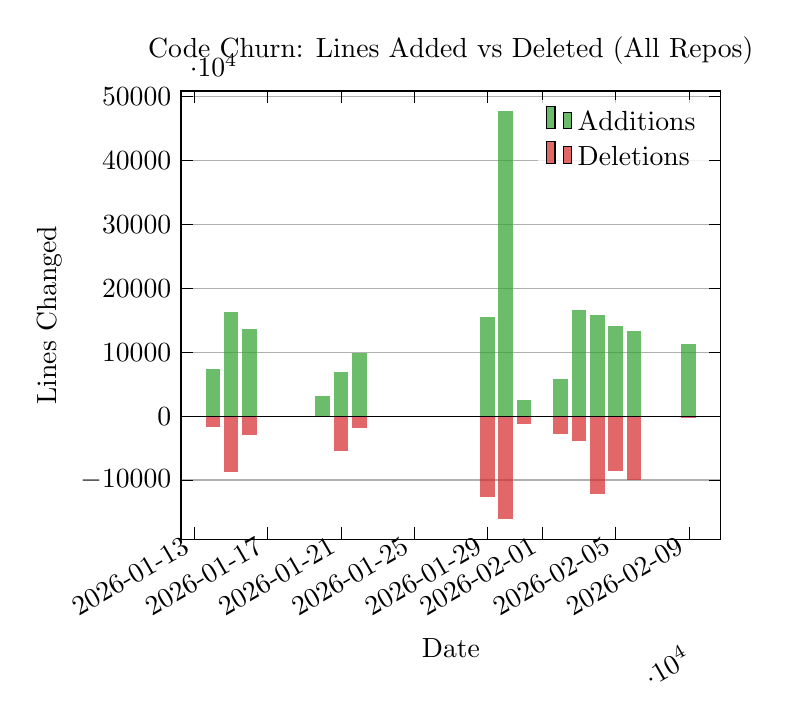
\begin{tikzpicture}

\definecolor{crimson2143940}{RGB}{214,39,40}
\definecolor{darkgray176}{RGB}{176,176,176}
\definecolor{forestgreen4416044}{RGB}{44,160,44}

\begin{axis}[
legend cell align={left},
legend style={fill opacity=0.8, draw opacity=1, text opacity=1, draw=none},
tick pos=both,
title={Code Churn: Lines Added vs Deleted (All Repos)},
x grid style={darkgray176},
xlabel={Date},
xmin=20465.26, xmax=20494.74,
xtick style={color=black},
xtick={20466,20470,20474,20478,20482,20485,20489,20493},
xticklabel style={rotate=30.0,anchor=east},
xticklabels={
  2026-01-13,
  2026-01-17,
  2026-01-21,
  2026-01-25,
  2026-01-29,
  2026-02-01,
  2026-02-05,
  2026-02-09
},
y grid style={darkgray176},
ylabel={Lines Changed},
ymajorgrids,
ymin=-19259.4, ymax=50841.4,
ytick style={color=black},
ytick={-20000,-10000,0,10000,20000,30000,40000,50000,60000},
yticklabels={
  \(\displaystyle {\ensuremath{-}20000}\),
  \(\displaystyle {\ensuremath{-}10000}\),
  \(\displaystyle {0}\),
  \(\displaystyle {10000}\),
  \(\displaystyle {20000}\),
  \(\displaystyle {30000}\),
  \(\displaystyle {40000}\),
  \(\displaystyle {50000}\),
  \(\displaystyle {60000}\)
}
]
\draw[draw=none,fill=forestgreen4416044,fill opacity=0.7] (axis cs:20466.6,0) rectangle (axis cs:20467.4,7389);
\addlegendimage{ybar,ybar legend,draw=none,fill=forestgreen4416044,fill opacity=0.7}
\addlegendentry{Additions}

\draw[draw=none,fill=forestgreen4416044,fill opacity=0.7] (axis cs:20467.6,0) rectangle (axis cs:20468.4,16322);
\draw[draw=none,fill=forestgreen4416044,fill opacity=0.7] (axis cs:20468.6,0) rectangle (axis cs:20469.4,13608);
\draw[draw=none,fill=forestgreen4416044,fill opacity=0.7] (axis cs:20472.6,0) rectangle (axis cs:20473.4,3149);
\draw[draw=none,fill=forestgreen4416044,fill opacity=0.7] (axis cs:20473.6,0) rectangle (axis cs:20474.4,6920);
\draw[draw=none,fill=forestgreen4416044,fill opacity=0.7] (axis cs:20474.6,0) rectangle (axis cs:20475.4,9920);
\draw[draw=none,fill=forestgreen4416044,fill opacity=0.7] (axis cs:20481.6,0) rectangle (axis cs:20482.4,15571);
\draw[draw=none,fill=forestgreen4416044,fill opacity=0.7] (axis cs:20482.6,0) rectangle (axis cs:20483.4,47655);
\draw[draw=none,fill=forestgreen4416044,fill opacity=0.7] (axis cs:20483.6,0) rectangle (axis cs:20484.4,2440);
\draw[draw=none,fill=forestgreen4416044,fill opacity=0.7] (axis cs:20485.6,0) rectangle (axis cs:20486.4,5856);
\draw[draw=none,fill=forestgreen4416044,fill opacity=0.7] (axis cs:20486.6,0) rectangle (axis cs:20487.4,16597);
\draw[draw=none,fill=forestgreen4416044,fill opacity=0.7] (axis cs:20487.6,0) rectangle (axis cs:20488.4,15814);
\draw[draw=none,fill=forestgreen4416044,fill opacity=0.7] (axis cs:20488.6,0) rectangle (axis cs:20489.4,14028);
\draw[draw=none,fill=forestgreen4416044,fill opacity=0.7] (axis cs:20489.6,0) rectangle (axis cs:20490.4,13352);
\draw[draw=none,fill=forestgreen4416044,fill opacity=0.7] (axis cs:20492.6,0) rectangle (axis cs:20493.4,11307);
\draw[draw=none,fill=crimson2143940,fill opacity=0.7] (axis cs:20466.6,0) rectangle (axis cs:20467.4,-1773);
\addlegendimage{ybar,ybar legend,draw=none,fill=crimson2143940,fill opacity=0.7}
\addlegendentry{Deletions}

\draw[draw=none,fill=crimson2143940,fill opacity=0.7] (axis cs:20467.6,0) rectangle (axis cs:20468.4,-8672);
\draw[draw=none,fill=crimson2143940,fill opacity=0.7] (axis cs:20468.6,0) rectangle (axis cs:20469.4,-3016);
\draw[draw=none,fill=crimson2143940,fill opacity=0.7] (axis cs:20472.6,0) rectangle (axis cs:20473.4,-139);
\draw[draw=none,fill=crimson2143940,fill opacity=0.7] (axis cs:20473.6,0) rectangle (axis cs:20474.4,-5441);
\draw[draw=none,fill=crimson2143940,fill opacity=0.7] (axis cs:20474.6,0) rectangle (axis cs:20475.4,-1877);
\draw[draw=none,fill=crimson2143940,fill opacity=0.7] (axis cs:20481.6,0) rectangle (axis cs:20482.4,-12689);
\draw[draw=none,fill=crimson2143940,fill opacity=0.7] (axis cs:20482.6,0) rectangle (axis cs:20483.4,-16073);
\draw[draw=none,fill=crimson2143940,fill opacity=0.7] (axis cs:20483.6,0) rectangle (axis cs:20484.4,-1182);
\draw[draw=none,fill=crimson2143940,fill opacity=0.7] (axis cs:20485.6,0) rectangle (axis cs:20486.4,-2727);
\draw[draw=none,fill=crimson2143940,fill opacity=0.7] (axis cs:20486.6,0) rectangle (axis cs:20487.4,-3957);
\draw[draw=none,fill=crimson2143940,fill opacity=0.7] (axis cs:20487.6,0) rectangle (axis cs:20488.4,-12120);
\draw[draw=none,fill=crimson2143940,fill opacity=0.7] (axis cs:20488.6,0) rectangle (axis cs:20489.4,-8576);
\draw[draw=none,fill=crimson2143940,fill opacity=0.7] (axis cs:20489.6,0) rectangle (axis cs:20490.4,-10032);
\draw[draw=none,fill=crimson2143940,fill opacity=0.7] (axis cs:20492.6,0) rectangle (axis cs:20493.4,-344);
\addplot [very thin, black, forget plot]
table {%
20465.26 0
20494.74 0
};
\end{axis}

\end{tikzpicture}
